\chapter{補間}
    \section{DTFT と IDTFT を用いた有限長信号の補間}
        \subsection{動機}
            有限長の離散時間信号(例えば係数畳み込み型 FIR フィルタ係数)が与えられたとき、その信号を連続時間信号に拡張して、任意の時刻での値を求めたいときがある。
            例えば FIR フィルタのインパルス応答が離散時間信号として既知であるとき、非整数の時刻に於ける合理的な値を考えたい(これはアップ・サンプリングの為の poly-phase フィルタの係数を計算する方法の一つである)。
        \subsection{方法}
            \label{DTFT と IDTFT を用いた有限長信号の補間の方法}
            台有界な離散時間信号 $\xd:\integers\to\complexNumbers$ の DTFT を $\Xd:\realNumbers\to\complexNumbers$ とする。
            但し引数は正規化角周波数である。
            連続時間信号 $\hat{x}:\realNumbers\to\realNumbers$ を次式で定義する。
            \[ \hat{x}(t)\coloneq\left.\IDTFT{\Xd}(n)\right|_{n\to t} = \frac{1}{2\pi}\integrate{-\pi}{\pi}{\Xd(\Omega)\exp\parens*{i\Omega t}}{}{\Omega} \]
            殆ど自明なことだが、$\hat{x}$ は全ての離散時刻に於いて $\xd$ と一致する連続関数である。
            \par
            例えば $\xd$ が既知であって、それをある時間 $d\in(0,1)$ だけ仮想的に遅らせた(サンプリング時刻が仮想的に $d$ だけ早まった)離散時間信号は $n\in\integers\mapsto\hat{x}(n-d)$ である。
            これも殆ど自明なことだが、この信号の DTFT のエネルギー・スペクトラム密度は $\xd$ のそれと等しい。
        \subsection{数値例}
            $N=33,\;\alpha=0.4$ とし、有限長の離散時間信号 $h:\integers\to\realNumbers$ を次式で定義する。
            これは視覚的な解り易さから \cite{learn_sp_from_basic} 式 (8.41) から流用したものである。
            \[
                h(n) = \begin{cases}
                    \alpha & (n=(N-1)/2) \\
                    \alpha\sinc{\parens*{(N-1)/2-\pi}\alpha\pi} & (n\in\{0,1,2,\dots,N-1\}\setminus\{(N-1)/2\}) \\
                    0 & (\text{otherwise})
                \end{cases}
            \]
            次の図は $h$ とその DTFT である。
            \begin{figure}[H]
                \centering
                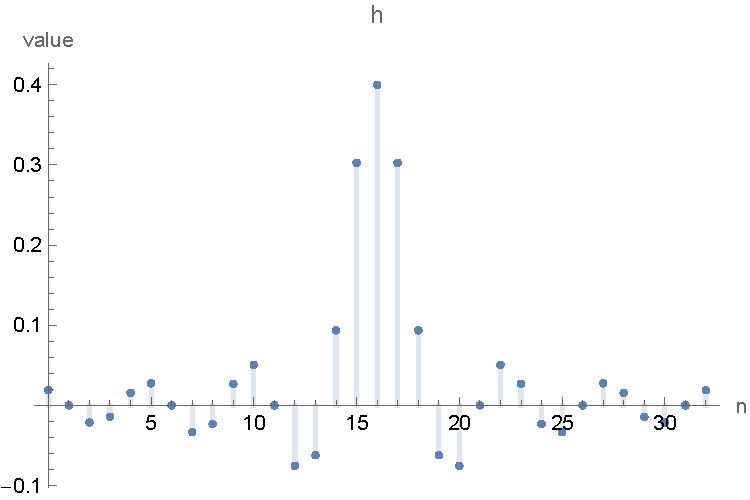
\includegraphics[keepaspectratio, scale=0.7]
                {\currfiledir/calc/Interpolation_with_DTFT_and_IDTFT/h.pdf}
                \caption{$h$}
            \end{figure}
            \begin{figure}[H]
                \centering
                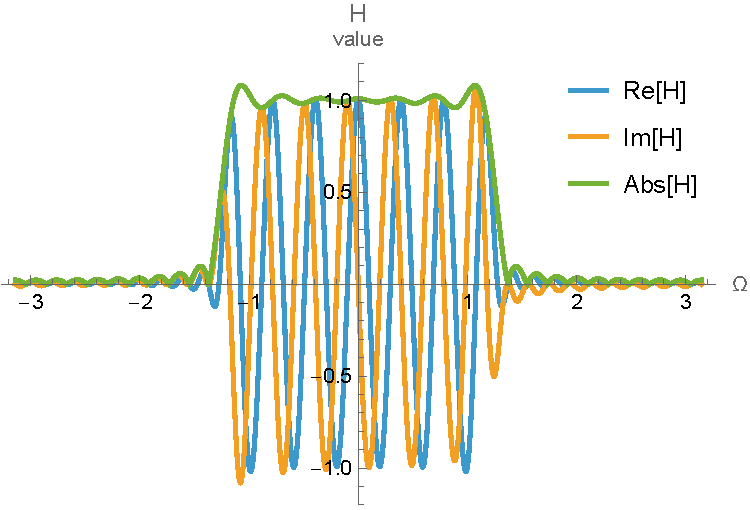
\includegraphics[keepaspectratio, scale=0.7]
                {\currfiledir/calc/Interpolation_with_DTFT_and_IDTFT/DTFT_of_h.pdf}
                \caption{$h$ の DTFT。横軸は正規化角周波数}
            \end{figure}
            これを前小節の方法で実時間信号に拡張したものを $\tilde{h}$ とする。
            次の図は $h$ と $\tilde{h}$ を重ねて描いたものである。
            \begin{figure}[H]
                \centering
                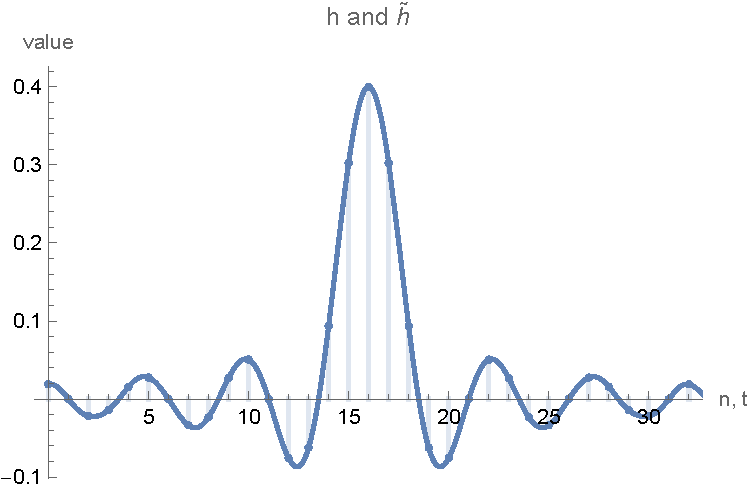
\includegraphics[keepaspectratio, scale=0.7]
                {\currfiledir/calc/Interpolation_with_DTFT_and_IDTFT/h_and_h_tilde.pdf}
                \caption{$h$ と $\tilde{h}$}
            \end{figure}
            新たな離散時間信号 $h^\dagger:(d,n)\in\realNumbers\times\integers\mapsto\tilde{h}(n-d)$ を定義する。
            $h^\dagger$ は $h$ を仮想的に $d$ だけ遅らせたものである。
            \begin{figure}[H]
                \centering
                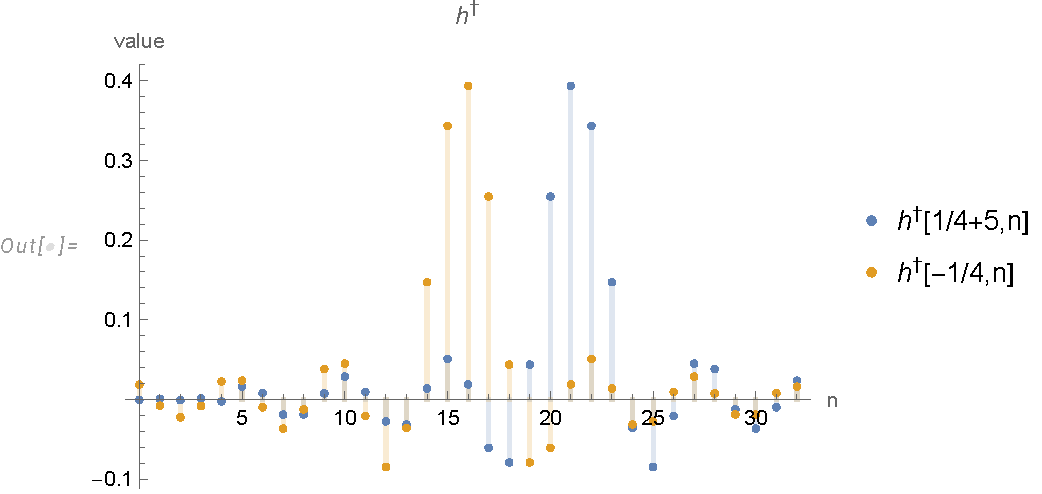
\includegraphics[keepaspectratio, scale=0.7]
                {\currfiledir/calc/Interpolation_with_DTFT_and_IDTFT/h_and_h_dag.pdf}
                \caption{$h^\dagger,\quad d=-0.25,\;0.75$}
            \end{figure}
            この数値例を計算した Mathematica notebook が下記のファイル名で保存されている。
            Git リポジトリ内でファイル名検索すれば発見できるであろう。
            notebook 中では前記 $N$ が \inlineCode{N_tp} となっている。\newline
            \href{\currfiledir/calc/Interpolation_with_DTFT_and_IDTFT/Interpolation_with_DTFT_and_IDTFT.nb}{Interpolation\_with\_DTFT\_and\_IDTFT.nb}\newline
        % \subsection{等間隔補間信号の周波数スペクトラム}
        %     \ref{DTFT と IDTFT を用いた有限長信号の補間の方法} で
